\documentclass[a5paper]{article}
\usepackage[a5paper, top=8mm, bottom=8mm, left=8mm, right=8mm]{geometry}

\usepackage{polyglossia}
\setdefaultlanguage[babelshorthands=true]{russian}
\usepackage{minted}

\usepackage{fontspec}
\setmainfont{FreeSerif}
\newfontfamily{\russianfonttt}[Scale=0.7]{DejaVuSansMono}

\usepackage[font=scriptsize]{caption}

\usepackage{amsmath}
\usepackage{amssymb,amsfonts,textcomp}
\usepackage{xcolor}
\usepackage{array}
\usepackage{hhline}
\usepackage{cite}
\usepackage{ulem}

\usepackage[xetex,linktocpage=true,plainpages=false,pdfpagelabels=false]{hyperref}
\hypersetup{colorlinks=true, linkcolor=blue, citecolor=blue, filecolor=blue, urlcolor=blue, pdftitle=1, pdfauthor=, pdfsubject=, pdfkeywords=}

\usepackage{tabu}

\usepackage{graphicx}
\usepackage{indentfirst}
\usepackage{multirow}
\usepackage{subfig}
\usepackage{footnote}
\usepackage{listings}

\newcommand{\attribution}[1] {
\vspace{-5mm}\begin{flushright}\begin{scriptsize}\textcolor{gray}{\textcopyright\, #1}\end{scriptsize}\end{flushright}
}

\sloppy
\pagestyle{plain}

\title{Практика 3: Объектно-ориентированное проектирование}

\date{29.01.2020}

\begin{document}

\maketitle
\thispagestyle{empty}

\section{Введение}

На этой лекции предлагается вернуться к азам и поговорить про объектно-ориентированное программирование: абстракцию, инкапсуляцию, наследование, полиморфизм и прочие связанные вещи. Это всё, конечно, изучают на первом курсе, но после пары лет опыта написания кода нелишне освежить знания в памяти и взглянуть на вещи с другой точки зрения. Так что сейчас будет довольно дискуссионная пара, где будут рассказаны вещи, которые вы и так знаете, но на сей раз рассказаны с архитектурной точки зрения. И можно будет обсудить некоторые моменты (для этого тут приготовлено несколько провокационных высказываний).

\section{Абстракция}

Начнём мы с абстракции. Принято считать, что основы ООП (``три кита ООП'') --- это инкапсуляция, наследование и полиморфизм. На самом деле, самым важным понятием ООП является \textit{абстракция}, хотя она и не относится к ``китам'' ООП, потому что она касается не только ООП, но и всего остального --- структурного, функционального программирования, алгебры и вообще способности людей к мышлению.

Рассмотрим пример. У нас есть объект ``Шрифт'' и мы хотим уметь менять ему размер. Вот так это можно было бы сделать:

\begin{itemize}
	\item \mintinline{java}|currentFont.size = 16| --- прямое присвоение полю, ужасно. Во-первых, шрифт не может поддерживать свой инвариант и изменить внутреннее представление размера. Во-вторых, тут написано ``размеру присвоить 16''. Окей, чего 16? Ну, а чего размеру?
	\item \mintinline{java}|currentFont.size = PointsToPixels(12)| --- чуть лучше. Теперь размер, видимо, измеряется в пикселях.
	\item \mintinline{java}|currentFont.sizeInPixels = PointsToPixels(12)| --- ещё чуть лучше. Теперь про размер явно написано, что он измеряется в пикселях.
	\item \mintinline{java}|currentFont.setSizeInPoints(sizeInPoints)| \newline
			\mintinline{java}|currentFont.setSizeInPixels(sizeInPixels)| --- совсем хорошо. Нам-то какое дело, в чём внутри у шрифта измеряется размер, мы хотим его выставлять в тех единицах измерения, которые нам удобны.
\end{itemize}

Ещё один небольшой пример, обычного класса на Java, который умеет, видимо, что-то исполнять и печатать по этому делу отчёты:

\begin{minted}{java}
public class Program {
    public void initializeCommandStack() { ... }
    public void pushCommand(Command command) { ... }
    public Command popCommand() { ... }
    public void shutdownCommandStack() { ... }
    public void initializeReportFormatting() { ... }
    public void formatReport(Report report) { ... }
    public void printReport(Report report) { ... }
    public void initializeGlobalData() { ... }
    public void shutdownGlobalData() { ... }
}
\end{minted}

Тут никаких полей нет, имена методов и параметров адекватны, но всё равно этот класс ужасен. Потому что нарушает принцип единственности ответственности. Он умеет и что-то делать со стеком команд, и с отчётами, и с глобальными данными, так что непонятно, когда и как им пользоваться. Про этот класс нельзя одним предложением сказать, что он такое. Чтобы сделать этот класс хорошим, его неплохо бы распилить на три --- стек команд, управлялка отчётами и хранилище глобальных данных. И добавить четвёртый класс, который бы управлял этими тремя классами. И это не будет овердизайном в стиле EnterpriseFizzBuzz, потому что тут и так на самом деле три класса, просто они упиханы в один.

Вот другой класс на Java, представляющий сотрудника какой-то компании:

\begin{minted}{java}
public class Employee {
    public Employee(
            FullName name,
            String address,
            String workPhone,
            String homePhone,
            TaxId taxIdNumber,
            JobClassification jobClass
    ) { ... }

    public FullName getName() { ... }
    public String getAddress() { ... }
    public String getWorkPhone() { ... }
    public String getHomePhone() { ... }
    public TaxId getTaxIdNumber() { ... }
    public JobClassification getJobClassification() { ... }
}
\end{minted}

У этого класса с абстракцией всё хорошо, он занимается ровно одним делом (представляет сотрудника компании), все имена понятны. Кроме того, тут используется ещё один хороший для абстракции приём --- специальные типы для значений. Например, TaxId вполне может быть классом с ровно одним полем типа String, геттером и сеттером, и всё. Зато теперь тут скрыто внутреннее представление TaxId (и его легко можно переделать на int, если окажется, что это возможно) и компилятор поругается, если мы перепутаем порядок аргументов. FullName может быть несколько более сложной штукой, там может быть фамилия, имя и отчество. Мы это всё тоже могли бы передавать в конструктор Employee как три отдельные строки, но зачем, ведь FullName --- это концептуально целостная штука. Достоинства такого подхода понятны, недостатки тоже --- за абстракцию и большую надёжность мы платим строками кода. Стоит ли платить эту цену --- приходится решать в каждом конкретном случае. Отмечу, что в функциональных языках объявить тип обычно гораздо менее трудозатратно, чем в Java, так что там таким приёмом пользуются часто и с удовольствием.

В продолжение темы платы строками кода за качество абстракции ещё один пример:

\begin{minted}{java}
public class Point {
    public double x;
    public double y;
}
\end{minted}

против

\begin{minted}{java}
public interface Point {
    double getX();
    double getY();
    void setCartesian(double x, double y);
    double getR();
    double getTheta();
    void setPolar(double r, double theta);
}
\end{minted}

Тут мы видим, что поскольку в Java нет структур, то приходится объявлять классы, и чтобы не писать ненужных геттеров/сеттеров, можно сразу объявить public-поля, потому что по смыслу это структура, инвариантов у неё нет, и использовать её предполагается только как хранилище данных. Тем не менее, несмотря на большую многословность, второй вариант более архитектурно правильный, потому что обладает интересным свойством --- тут вообще нигде не написано, как точка представляется внутри. Мы можем трактовать точку как точку в декартовых координатах, можем --- как в полярных, ей всё равно. Для этого, кстати, геттеры позволяют получить каждую координату отдельно, но сеттеры позволяют выставить только обе координаты сразу --- позволять менять координаты по одной было бы странно с точки зрения семантики операций с учётом того, что изначально точка могла задаваться в другой системе координат. Кстати, этот пример показателен не только для Java, где всё очень плохо, но и для C\#, где есть и структуры и свойства --- первая абстракция всё равно отличается от второй тем, что она ``недостаточно абстрактна''. Нужна ли нам большая абстрактность или это приведёт к очередному EnterpriseFizzBUzz с его абстрагированием цикла --- вопрос, на который должен ответить архитектор, опять-таки, для каждого конкретного случая.

Вообще, объектно-ориентированое программирование и структуры находятся в довольно странных отношениях. Структуры и классы более-менее взаимозаменаемы, с учётом следующих соображений:

\begin{itemize}
	\item объекты скрывают свои данные за абстракциями и предоставляют функции для работы с ними;
	\item структуры раскрывают данные и не имеют осмысленных функций.
\end{itemize}

При этом,
\begin{itemize}
	\item процедурный код позволяет легко добавлять новые функции без изменения существующих структур данных;
	\item объектно-ориентированный код, напротив, упрощает добавление новых классов без изменения существующих функций.
\end{itemize}

Хороший пример использования структур в объектно-ориентированном (ну, более-менее) коде --- списки в стандартной библиотеке языка F\#. Список представляется классом list, который имеет ровно 7 методов (плюс методы реализуемых им четырёх интерфейсов), методы Head, IsEmpty, Item(int), Length, Tail и два статических метода Cons и Empty. Тип Collections.List, который в этой же библиотеке, имеет больше 60 статических методов, принимающих объекты типа list и делающие с ними всякие вещи типа filter, fold, map, sum и т.д. Фактически list выступает как структура, хранящая данные, List --- как набор функций, с этими данными работающий. Такой же приём применялся для объектно-ориентированного программирования в языке Ада, там тоже структура с данными была отдельно и её надо было явно передавать в методы (может и сейчас там так, может нет, там относительно недавно выходил новый стандарт).

Следующее соображение, влияющее на качество абстракции --- это её ``уровень'' и консистентность этого уровня по абстракции. Например:

\begin{minted}{java}
public class EmployeeRoster implements MyList<Employee> {
    public void addEmployee(Employee employee) { ... }
    public void removeEmployee(Employee employee) { ... }
    public Employee nextItemInList() { ... }
    public Employee firstItem() { ... }
    public Employee lastItem() { ... }
}
\end{minted}

Тут принцип единственности ответственности соблюдается --- это список сотрудников какой-то компании, всё хорошо. Наследование используется по делу, список сотрудников определённо является списком. Имена и параметры тоже адекватны --- можно добавить сотрудника, получить сотрудника, удалить сотрудника, вроде всё ок. Тем не менее, сравним это со вторым классом:

\begin{minted}{java}
public class EmployeeRoster {
    public void addEmployee(Employee employee) { ... }
    public void removeEmployee(Employee employee) { ... }
    public Employee nextEmployee() { ... }
    public Employee firstEmployee() { ... }
    public Employee lastEmployee() { ... }
}
\end{minted}

Тут мы уже не наследуемся от списка (о ужас, теперь для нашего класса не будут работать библиотечные алгоритмы, работающие над списками) и переименовали пару методов. Стало лучше? Гм, рассмотрим ещё один пример --- в стандартной библиотеке Java долгое время стек наследовался от списка. Ну а что, стек --- это список с методами push и pop. Теперь это каноничный пример плохого дизайна --- стек, конечно, не список, потому что не должен получать от списка пачку методов, ломающих инварианты стека. Но суть даже не в инвариантах, а в том, что стек --- это что-то простое, список --- это что-то сложное и предназначенное не для того. Возвращаясь к нашему примеру, список сотрудников --- это что-то сложное и техническое, у него есть методы для итерирования (nextItemInList, firstItem и lastItem) и мало ли что ещё. А мы хотим просто список сотрудников, мы не хотим итератор (может, мы двенадцатилетний сын директора компании, который пишет на Питоне автоматизацию начисления зарплаты). Поэтому хорошая абстракция часто вынуждена не расширять уже существующую, а прятать её и предоставлять более простой интерфейс, даже несмотря на то, что это усложнит переиспользование кода. Задача абстракции --- быть удобной для использования и для понимания, а не уметь делать много всего. При этом удобство понимания важнее.

Есть некоторый набор общих рекомендаций, про которые тоже неплохо бы помнить, проектируя свои классы и интерфейсы.

\begin{itemize}
	\item Про каждый класс знайте, реализацией какой абстракции он является. Принцип единственности ответственности имеет очень простой критерий --- если про класс можно одним коротким предложением сказать, что он такое, то всё ок. Может потребоваться разделить класс на несколько разных классов просто потому, что методы по смыслу слабо связаны, и это будет не овердизайн, как мы видели ещё в первом примере.
	\item Учитывайте противоположные методы (add/remove, on/off, ...). Даже если они сейчас не нужны, когда-то кому-то неизбежно понадобятся.
	\item Разделяйте команды и запросы, избегайте побочных эффектов. Команда только меняет состояние, не возвращая результат, запрос только возвращает результат, не меняяя состояния. Это хорошо как для понимания программы, так и по более прагматичному соображению --- в многопоточной программе синхронизации требуют только команды. Сколько угодно запросов может исполняться параллельно.
	\item Не возвращайте null. null всегда сюрприз для вызывающего, даже если он прекрасно знает, что любой ссылочный тип может иметь значение null. Возвращайте Option --- это вынудит вызывающего явно проверить наличие значения. Ну или бросайте исключение, если null-ы бывают только если что-то пошло не так.
	\item По возможности делайте некорректные состояния невыразимыми в системе типов. Это особо хорошо работает в функциональных языках, потому что там мощные системы типов, но и в других языках систему типов можно заставить работать на себя --- вспомните второй пример, с TaxId и FullName у Employee.
	\item Семантику языка тоже надо заставить работать на себя в плане чистоты абстракций. Самый простой пример --- комментарии в духе ``не пользуйтесь объектом, не вызвав  init()'' можно заменить конструктором. Вообще, всё, что не проверяется компилятором, будет использовано неправильно, так что надо стараться так, чтобы вашей абстракцией пользоваться неправильно было просто невозможно.
	\item При рефакторинге надо следить, чтобы интерфейсы не деградировали. Рефакторинг --- опасная вещь, потому что в погоне за тактической выгодой типа скорости работы или удобства вызовов можно потерять стратегические преимущества хороших абстракций.
\end{itemize}

\section{Инкапсуляция}

Следующее важное понятие в ООП --- это инкапсуляция. Под которым обычно понимают сокрытие деталей реализации, несмотря на то, что инкапсуляция --- это обычно просто свойство кода, относящегося к одной задаче, лежать рядом. В принципе, в ООП и инкапсуляция в этом понимании, и сокрытие деталей реализации обеспечиваются классами (либо чем-то похожим), так что всё вместе называть инкапсуляцией вполне валидно.

Инкапсуляция --- это механизм защиты инвариантов объекта на самом деле. Из этого следует, во-первых, принцип минимизации доступности методов, который коротко формулируется как ``меньше знаешь --- крепче спишь''. Чем меньше интерфейс объекта, тем проще им пользоваться и тем проще уследить за инвариантами объекта. С другой стороны, тем меньше объект умеет делать, но это даже хорошо --- принцип единственности ответственности и всё такое. Другое дело, что если у всех объектов ровно по одному методу (как в функциональных программах, например), то это не идеальная инкапсуляция, а наоборот печаль, потому что сложность переносится из объектов во взаимодействие между объектами.

Во-вторых, из этого следует, что паблик-полей не бывает. Паблик-поля вообще не могут поддерживать никаких инвариантов, поэтому, скорее всего, просто не относятся к тому классу, в котором объявлены. Это, конечно, вызывает вопросы ``А что делать, если класс не имеет инвариантов и так, например, используется только для передачи данных?''. Например,

\begin{minted}{java}
class Point {
    public float x;
    public float y;
    public float z;
}
\end{minted}

и

\begin{minted}{java}
class Point {
    private float x;
    private float y;
    private float z;
    public float getX() { ... }
    public float getY() { ... }
    public float getZ() { ... }
    public void setX(float x) { ... }
    public void setY(float y) { ... }
    public void setZ(float z) { ... }
}
\end{minted}

По этому поводу бывают разные мнения, во многих языках есть структуры специально для таких дел, но в целом сообщество сходится на том, что второй вариант предпочтительнее, несмотря на то, что его стоимость в строках кода в разы выше. Почему --- код, к несчастью, имеет свойство развиваться, так что то, что раньше было просто классом для передачи данных без инвариантов или чего бы то ни было, внезапно становится полноценной абстракцией с кучей методов, инвариантов и т.д. и т.п. Геттеры с сеттерами легко подправить так, чтобы они начали делать что-то умное, поля --- придётся переписывать весь код, использующий наш класс.

В C++ есть один известный приём, который позволяет скрыть детали реализации абсолютно --- Pointer To Implementation (идиома ``Pimpl''). Идея в том, что вместо хранения даже private-полей в классе-абстракции мы в классе храним только одно поле --- указатель на класс-реализацию. Класс-реализация описывается только в соответствующем .cpp-файле, поэтому по правилам компиляции кода на C++ вообще не виден никому, кроме его класса-абстракции. Класс-абстракция объявляет только методы, и все методы просто делегируют запрос классу-реализации, который и делает полезную работу. Зачем --- дело в том, что в C++ всё очень плохо с модульностью, поэтому там если мы даже в private-части определения класса используем какие-то типы, размер этих типов должен быть известен во время компиляции всего кода, который хочет использовать наш класс. Например,

\begin{minted}{c++}
class Employee {
public:
    Employee(...);
    std::string name() const;
    std::string surname() const;
    std::string address() const;
private:
    FullName mName;
    std::string mAddress;
    int mJobClass;
};
\end{minted}

Тут всем, кто хочет пользоваться классом Employee, придётся ещё и знать про класс FullName (и подключать его объявление вместе с объявлением Employee). Что, во-первых, негативно сказывается на зависимостях при компиляции и вообще связности программы, во-вторых, тупо увеличивает время компиляции, потому что Employee может быть подключен в тысяче файлов, так что FullName (и все его зависимости тоже) придётся скомпилить тысячу раз заново (вообще в C++ есть механизм precompiled headers, но он имеет ряд проблем, поэтому им обычно пользуются с осторожностью, да и при первой компиляции это не помогает). Решение с помощью Pointer To Implementation:

\begin{minted}{c++}
class EmployeeImplementation;

class Employee {
public:
    Employee(...);
    std::string name() const;
    std::string surname() const;
    std::string address() const;
private:
    EmployeeImplementation *mImpl;
};
\end{minted}

Ну и в EmployeeImplementation в .cpp-файле пишем то же, что раньше у нас было в Employee. Теперь ничего подключать не надо, кроме того, что используется в интерфейсной части Employee и и так должно быть доступно его пользователям. Такой приём громоздок, противоестественен и усложняет отладку, но многие библиотеки (например, Qt) используют его очень активно, поскольку он позволяет менять реализацию, не затрагивая интерфейс, не ломая бинарную совместимость и т.д. Это сродни интерфейсу плюс фабрике в более ОО-языках типа Java или C\#.

Ещё некоторые рекомендации касательно инкапсуляции.

\begin{itemize}
	\item Лёгкость чтения кода важнее, чем удобство его написания. Написать код надо один раз (при этом IDE будет помогать всякими автодополнениями), а читать его придётся, быть может, тысячи раз разным людям.
	\item Класс не должен ничего знать о своих клиентах. Образ мыслей ``а здесь я не буду вставлять проверку на null, потому что из моего кода его никто с null не вызывает'' неправильный, это нарушение инкапсуляции ``с другой стороны'' (когда не внешний мир лезет в класс, а класс чего-то хочет от внешнего мира). Всё сломается, когда ваш класс захотят переиспользовать где-то ещё.
	\item Опасайтесь семантических нарушений инкапсуляции, например, ``не будем вызывать ConnectToDB(), потому что GetRow() сам его вызовет, если соединение не установлено''. Даже если это правда, это предположение о том, как реализована абстракция, или программирование \textit{сквозь} интерфейс.
	\item Protected- и package- полей тоже не бывает. На самом деле, у класса два интерфейса --- для внешних объектов и для потомков (может быть отдельно третий, для классов внутри пакета, но это может быть плохо). Все эти интерфейсы должны быть полноценными интерфейсами, то есть защищать инварианты, поддерживать контракты и т.д. Потомков вы вообще не контролируете и доверять им нельзя, классы внутри пакета безопаснее, но тоже никто не сказал, что ваш пакет будете всегда разрабатывать только вы и только в непомутнённом состоянии рассудка.
\end{itemize}

Ещё один важный аспект инкапсуляции --- это инкапсуляция чужого кода. Вообще, чудой код и так должен быть инкапсулирован, если это адекватный код, но иногда полезно иметь вокруг него ещё один слой инкапсуляции. Например, чтобы ваша система не зависела от конкретной библиотеки конкретного поставщика и её можно было легко поменять. Во-вторых, чтобы защитить свой код от изменений в третьестороннем коде (по этому поводу я видел в одной из рекомендованных ниже книжек страшную историю про стандартную библиотеку Java и её класс HashMap, который в какой-то из релизов сильно поменялся, так что наученные горьким опытом разработчики с тех пор писали свои обёртки над подозрительными классами из стандартной библиотеки). В-третьих, чтобы упростить сложное API стороннего кода. Довольно типичный пример такой инкапсуляции --- слой доступа к данным, когда всё общение с конкретной БД выносится в отдельные классы, реализующие чётко прописанный интерфейс, чтобы можно было легко поменять БД, если станет нужно. При этом интерфейс обычно описан в терминах объектов из предметной области, а не абстрактных понятий из мира баз данных, для удобства работы.

Полезный приём при работе со сторонними API --- писать ``учебные тесты'', то есть юнит-тесты на чужую функциональность. В отличие от обычных юнит-тестов, цель учебных тестов не найти баги, а служить примером использования API и средством для экспериментирования и симуляции разных ``странных'' ситуаций, поведение API в которых может быть интересно. Учебные тесты имеет смысл не выкидывать когда вы полностью разобрались с библиотекой, с которой собираетесь интегрироваться --- они позволят вовремя заметить важные изменения в следующей версии сторонней библиотеки.

Есть даже паттерн проектирования, предназначенный прежде всего для интеграции чужого кода --- паттерн ``Адаптер''. Он позволяет сделать так, чтобы объект из сторонней библиотеки (от которого у вас, возможно, даже нет исходников) как буто реализовывал тот интерфейс, который вам нужен. Общая идея такая, что заводится класс-адаптер, который реализует нужный интерфейс и делегирует все запросы адаптируемому классу, возможно, выполняя необходимые преобразования и пред/пост-обработку.

\section{Наследование и полиморфизм}

Наследование хоть и считается одним из трёх китов, на которых зиждется ООП, современная архитектурная мысль считает его очень нишевым и довольно неуклюжим инструментом. Наследование почти всегда может быть заменено на агрегацию с делегированием запросов агрегируемому объекту, и на самом деле внутри в большинстве языков программирования наследование реализуется именно так --- класс-потомок просто имеет внутри себя объект класса-предка, методы которого можно вызывать по интерфейсу потомка. Агрегация или композиция имеют ряд преимуществ над наследованием, основное из которых --- возможность переконфигурирования во время выполнения. Наследование фиксируется во время компиляции и требуется перекомпилировать программу, чтобы поменять предка, в поле можно просто положить новый объект прямо в процессе работы. Даже во время компиляции наследование не очень гибко --- в разных языках есть ограничения на количество классов-предков, всякое ромбовидное наследование и тонкости, с ним связанные, и т.д. Агрегация лишена этих недостатков. У агрегации тоже есть проблемы --- во-первых, это чисто синтаксически необходимость явно описывать в нашем классе все методы, которые мы хотим поддержать, и реализовывать их перенаправлением запроса агрегируемому объекту (опять-таки, больше строк кода). Во-вторых, с агрегацией не работает полиморфизм (хотя если сам агрегируемый объект полиморфный, можно добиться ряда занятных эффектов, см. паттерны ``Состояние'' и ``Стратегия'').

Поэтому в целом можно сказать, что наследование имеет смысл использовать только для обеспечения полиморфизма. Наследование для переиспользования общей функциональности предка можно смело заменять на включение этого ``предка'' как поля во все классы, которым нужна его функциональность. А это, в свою очередь, значит, что наследоваться от конкретных (и даже абстрактных) классов нет никакой нужды --- интерфейсов для обеспечения полиморфизма вполне достаточно, а переиспользовать код предка всё равно плохо. Из этого, в свою очередь, следует, что private-наследование, как оно реализовано в C++, суть ересь. И C++ настолько ужасен, что наследование в нём private по умолчанию. Впрочем, по моему опыту, private-наследование в реальном промышленном коде на C++ используется крайне редко.

На самом деле, заявления выше несколько категоричны. Есть способы использования наследования для обеспечения конфигурирования класса-предка --- см., например, паттерн ``Шаблонный метод'' или большинство оконных библиотек. Там основная функциональность реализуется в классе-предке, потомки нужны, чтобы переопределить виртуальные методы предка так, чтобы всё вместе делало что-то полезное. Впрочем, большинство таких вещей писалось до массового распространения лямбда-функций в языках программирования, так что по-другому делать было просто очень неудобно. Возможно, мы скоро увидим фреймворки, которые наследованием не пользуются вовсе.

Наследование --- по определению отношение ``является'' между типами. Есть простой способ проверки иерархии наследования на адекватность --- принцип подстановки Барбары Лисков: любой код, который может работать с предком, должен мочь работать и с потомком. То есть наследование --- это наследование интерфейса (в смысле обеспечения полиморфизма подтипов), причём интерфейса в широком смысле --- обязательств и инвариантов.

Многие языки позволяют явно запретить наследование (final- или sealed-классы, final-методы). Есть две школы мысли по поводу того, как это использовать. Некоторые библиотекописатели (например, Microsoft) считают, что в библиотечном коде запрещать наследование нельзя, потому что это существенно ограничивает гибкость. Где-то в документации от Microsoft приводился пример с подключением к базе данных, где наследование от библиотечного класса использовалось только для того, чтобы определить конструктор, подставляющий нужный Connection String, и это типа удобно. Некоторые наоборот считают, что всё, для чего наследование не разрешено явно, должно быть закрыто для наследования, потому что если вы хотите позволить наследоваться от вашего класса, вам надо подумать о защите ваших инвариантов от потомков, о правильном использовании потомками методов вашего класса и т.д., это некоторая работа и делать её для каждого класса смысла нет.

Некоторые code smells, которые намекают на то, что с иерархией наследования что-то не так:

\begin{itemize}
	\item базовый класс, у которого только один потомок; оставлять возможности для расширения ``на будущее'', которое никогда не наступит, не стоит, благо в будущем можно и отнаследоваться, если будет надо, это не страшный рефакторинг;
	\item пустые переопределения --- предок декларирует контракты, которые потомок не может содержательно выполнить;
	\item очень много уровней в иерархии наследования --- обычно больше семи уровней означает, что всё совсем плохо, три-четыре уровня --- подозрительно; бывают исключения, например, иерархия наследования в абстрактном синтаксическом дереве компилятора;
	\item новые методы с такими же именами, как у родителей --- во-первых, это путает пользователя, во-вторых, это сильный индикатор того, что потомок вовсе потомком не является, а делает что-то своё.
\end{itemize}

Бывает, что наследование не используется там, где использоваться должно бы. Самый явный индикатор этого --- switch или длинная цепочка из if-else, где в зависимости от значения какого-то поля выбирается какое-то действие. Это на самом деле попытка реализовать вручную таблицу виртуальных методов. Простой пример:

\begin{minted}{java}
class Operation {
    private char sign = '+';
    private int left;
    private int right;

    public int eval() {
        switch (sign) {
            case '+': return left + right;
            case '-': return left - right;
        }
        throw new RuntimeException();
    }
}
\end{minted}

Это легко можно заменить на виртуальный вызов, где роль того поля, по которому делается выбор, играет тип времени выполнения объекта, у которого этот виртуальный вызов делается:

\begin{minted}{java}
abstract class Operation {
    private int left;
    private int right;

    protected int getLeft() { return left; }
    protected int getRight() { return right; }
    abstract public int eval();
}

class Plus extends Operation {
    @Override public int eval() { 
        return getLeft() + getRight(); 
    }
}

class Minus extends Operation {
    @Override public int eval() { 
        return getLeft() - getRight(); 
    }
}
\end{minted}

Опять-таки, кода становится больше, но архитектура в целом становится лучше --- теперь нет switch-а, который вынужден знать про все возможные операции, набор операций несложно расширить, теперь они могут быть довольно сложными (вплоть до того, чтоы собираться из элементарных операций в рантайме, см. паттерн ``Интерпретатор''). И операции в процессе развития программы могут получить ещё какую-нибудь ответственность, например, ``печатать себя'', и это будет очень легко поддержать, не городя ещё один гигантский switch.

\section{Вопросы инициализации}

Особого внимания заслуживают вопросы создания и инициализации объектов (и, что более интересно, сложных конструкций из нескольких объектов). Касательно конструкторов рекомендации такие:

\begin{itemize}
	\item Инициализируйте все поля, которые надо инициализировать. Конструктор --- это тот код, который более-менее обязательно выполняется при создании объекта, поэтому его задача --- сделать так, чтобы все инварианты после него выполнялись. Надеяться на то, что пользователь честно-честно вызовет метод init() после конструктора --- бессмысленно.
	\item Не вызывайте виртуальные методы из конструктора. Обычно вам даже компилятор скажет, что вы неправы, но если нет, последствия могут быть печальны. Дело в том, что при создании объекта конструкторы вызываются по цепочке, соответствующей иерархии наследования, при этом сначала вызываются конструкторы предка. Так что если ваш любимый язык таки позволяет сделать виртуальный вызов, вызовется метод потомка ещё до того, как конструктор потомка будет иметь шанс установить свои инварианты.
	\item Используйте private-конструкторы для объектов, которые не должны быть созданы или одиночек (некоторые языки позволяют явно сказать, что конструктора нет --- \mintinline{cpp}|= delete;| в C++, abstract в C\# и Java), protected-конструкторы для абстрактных классов --- создать их всё равно нельзя, так что нечего смущать пользователя, но из потомков вызывать конструктор может быть нужно.
	\item Одиночек надо использовать с большой осторожностью, потому как это замаскированные глобальные переменные со всеми вытекающими проблемами.
	\item Deep copy предпочтительнее Shallow copy, хотя второе может быть эффективнее. Пользователи в любом случае ожидают семантику глубокого копирования и могут быть удивлены, если изменения одного объекта приведут к изменению и другого. Глубокое копирование может быть сложным в реализации, если речь идёт про большой граф объектов, особенно если надо разбираться с идентичностью объектов (если объекты хранятся в БД или передаются по сети, их идентичность определяется не их местом в памяти, так что о ней надо думать при копировании). Если с идентичностью проблем нет, можно использовать такой хак --- сериализовать копируемый объект в поток байт в памяти, потом десериализовать.
\end{itemize}

Если вы создаёте один объект, проблем с его созданием немного. Но если речь идёт о создании и инициализации целой подсистемы, логика создания может стать довольно запутанной. В таком случае есть смысл вынести логику создания и инициализации в специально предназначенное для этого место, чтобы избавить классы, занимающиеся полезным делом, от несвойственной им и сложной функциональности по созданию объектов. В простых случаях может помочь паттерн ``Абстрактная фабрика'':

\begin{center}
	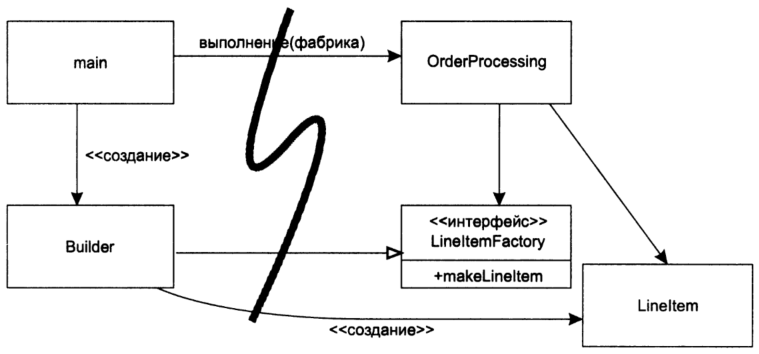
\includegraphics[width=0.7\textwidth]{factory.png}
	\attribution{Р. Мартин, Чистый код}
\end{center}

Тут логика создания объекта вынесена в отдельный класс Builder, который реализует интерфейс LineItemFactory с единственным методом makeLineItem, который возвращает новый объект LineItem. В принципе, фабрика может создавать несколько разных объектов, и не только создавать, но десериализовывать их, выстраивать из них сложные структуры, отдавая вызывающему целый граф объектов, уже проинициализированный и с выполняющимися инвариантами. Фабрику же можно передать и в ``боевой'' код, чтобы тот имел возможность создавать новые объекты по ходу работы, не думая, как ему их создавать. Ещё, кстати, фабрика позволяет не имет зависимости от конкретных типов во время компиляции, тогда как вызов конструктора обязательно требует знать конкретный тип. Так что фабрика способствует снижению связности.

В несколько более сложных случаях может помочь паттерн ``Строитель'':

\begin{center}
	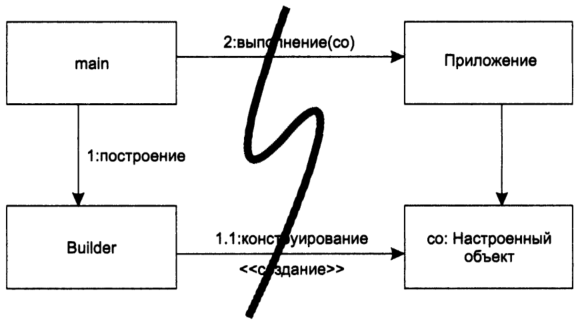
\includegraphics[width=0.7\textwidth]{builder.png}
	\attribution{Р. Мартин, Чистый код}
\end{center}

Строитель позволяет реализовать более сложную логику построения и настройки объекта (или целой группы объектов), разделяя собственно алгоритм построения и действия, выполняемые на каждом этапе построения объекта. Самый простой пример строителя --- класс StringBuilder из любой уважающей себя стандартной библиотеки. Ему можно передать несколько строк, которые надо сконкатенировать (в каком порядке и какие строки, определяет клиентский код --- Director в терминологии паттерна), а потом получить желаемую строку. При таком подходе main создаёт строитель и заставляет его по этапам строить структуру объектов, затем забирает из строителя готовый объект и отдаёт его ``боевому'' коду.

Если жизненный цикл объектов и их инициализация слишком сложны даже для фабрики и строителя, применяется тяжёлая артиллерия --- Dependency Injection. DI предполагает поддержание \textit{контейнера}, который следит за жизнью объектов, создаёт их при необходимости и выдаёт по запросу, сам проводя их инициализацию, в том числе устанавливая связи между создаваемым объектом и другими объектами из контейнера.

Самый простой способ сделать что-то такое --- это реестр объектов:

\begin{minted}{java}
MyService myService = (MyService)(jndiContext.lookup("NameOfMyService"));
\end{minted}

Кто-то (например, main) создаёт объекты и регистрирует их в реестре, дальше любой код, который имеет ссылку на реестр, может запросить из него созданный и проинициализированный объект. Например, там часто хранят объект, отечающий за доступ к базе данных --- создавать его каждый раз при необходимости неэффективно, потому что требуется заново устанавливать подключение к базе, нужен он много где, так что его один раз создают, регистрируют и отдают всем желающим по запросу. Реестр вполне может быть одиночкой, со всеми вытекающими негативными эффектами глобальных переменных, но база данных и так по сути глобальная переменная, так что сильно плохо от этого не будет.

Реестр объектов не умеет инициализировать объекты, поэтому \textit{IoC-контейнеры} идут дальше. Ведь можно руками вообще ничего не делать, просто сказать контейнеру, где лежит байт-код с классами, и запрашивать объект нужного типа. Он сам вполне может создать объект рефлексией. Но у создаваемого объекта могут быть свои зависимости, например, принимаемые как параметры конструктора --- тогда IoC-контейнер пытается создать объекты классов, которые нужны как параметры, и проинициализировать их, рекурсивно. В реальной жизни всё не так просто, потому что у объектов бывает разный жизненный цикл --- кто-то должен быть один на всю систему, кто-то должен создаваться каждый раз заново при каждом запросе. Ещё бывают конфигурационные параметры, типа connection string для подключения к СУБД. Всё это (и даже больше) умеют библиотечные контейнеры, поэтому их часто используют в больших системах для инициализации всего, что можно.

Пример такой библиотеки --- IoC-контейнеры Spring. Вообще, Spring --- это фреймворк для Java, предназначенный прежде всего для разработки распределённых приложений, веб-приложений и т.д., но умеющий уже практически что угодно. Там, как и у всех подобных библиотек, есть собственная подсистема IoC и Dependency Injection (интересно, кстати, что библиотеки, реализующие подход Dependency Injection, называют Inversion of Control Containers). Концептуально IoC в Spring принимает на вход реализации бизнес-объектов и конфигурационную информацию, выдавая сконфигурированную систему из объектов:

\begin{center}
	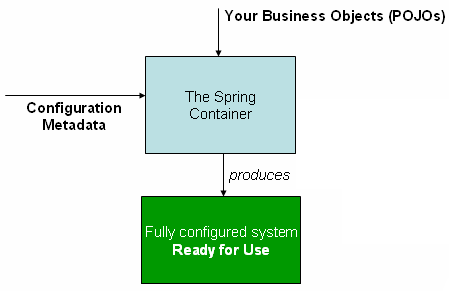
\includegraphics[width=0.5\textwidth]{springIoC.png}
\end{center}

Небольшой пример, стековый калькулятор. Положим, у нас есть класс ``Калькулятор'', выполняющий стековые вычисления. Ему можно передать выражение в виде строки в обратной польской записи, он, используя стек, посчитает значение этого выражения (как обычно, видим операнд --- кладём на стек, видим оператор --- снимаем операнды со стека, выполняем операцию, кладём результат на стек). Мы не хотим, чтобы калькулятор зависел от конкретной реализации стека (мало ли мы хотим попробовать стек на массиве, стек на указателях). Поэтому калькулятор будет знать только про интерфейс ``Stack'', реализацию которого будет принимать в конструктор:

\begin{minted}{java}
package ru.spbu.se.ioc;

public class Calculator {

    private Stack stack;

    public Calculator(Stack stack) {
        this.stack = stack;
    }

    public double calculate(String expression) {
        ...
        return stack.pop();
    }
}
\end{minted}

И сам интерфейс:

\begin{minted}{java}
public interface Stack {
    void push(double value);
    double pop();
    boolean isEmpty();
}
\end{minted}

И реализация (ну, я думаю, каждый может её сделать):

\begin{minted}{java}
public class LinkedStack implements Stack {
    ...
    ...
}
\end{minted}

Теперь, чтобы собрать всё воедино, надо сказать IoC-контейнеру, какую реализацию для чего использовать:

\begin{minted}{xml}
<?xml version="1.0" encoding="UTF-8"?>
<beans ....>

    <bean id="stack"
          class="ru.spbu.se.ioc.LinkedStack"
          />

    <bean id="calculator"
          class="ru.spbu.se.ioc.Calculator">
        <constructor-arg ref="stack"/>
    </bean>

</beans>
\end{minted}

Тут написано, что у нас есть класс LinkedStack, и что классу Calculator в конструктор надо передать именно его.

Сама магия происходит в main-е:

\begin{minted}{java}
public class Main {
    public static void main(String[] args) {
        ApplicationContext context = 
            new FileSystemXmlApplicationContext("config.xml");

        Calculator calculator = 
            context.getBean("calculator", Calculator.class);

        double result = calculator.calculate("1 2 + 3 *");
        System.out.println(result);
    }
}
\end{minted}

Мы создаём ApplicationContext (тот самый контейнер), говорим ему, где взять конфиг и просим создать экземпляр класса Calculator. Он смотрит в конфиг и создаёт стек, передаёт его во вновь созданный калькулятор, результат возвращает нам. Мы нигде в  коде вообще не вызываем никаких конструкторов. Странная терминология ``bean'' и getBean пришла из глубокой истории Java и попытки сделать там хорошую поддержку компонентов --- Java Beans. С компонентно-ориентированной разработкой не сложилось, но традиция называть биизнес-объекты bean-ами всё ещё жива.

\section{О мутабельности}

Мутабельность --- способность объекта изменять своё состояние --- довольно важное свойство, оказывающее существенное влияние на архитектуру. Если кратко, то мутабельное состояние --- это плохо и его надо стараться избегать. Более подробно, мутабельность запутывает причинно-следственные связи в программе --- кто-то вызвал метод, меняющий состояние, потом кто-то ещё, потом объект ведёт себя не так, как ожидалось. Кроме того, мутабельность создаёт дополнительные сложности для многопоточного программирования --- если состояние можно изменять, надо следить, чтобы два потока не пытались его изменить одновременно.

Тем не менее, основные современные языки программирования предполагают, что состояние мутабельно по умолчанию, а иногда (например, в Java) надо ещё помучаться, чтобы сделать класс немутабельным. Вот про что надо помнить, делая немутабельный класс.

\begin{itemize}
	\item Не предоставлять методы, модифицирующие состояние. Часто модификация состояния по смыслу всё-таки нужна, но есть полезный приём --- заменить модифицирующие состояние методы на методы, возвращающие копию объекта. При этом, разумеется, поменяется семантика программы, так что это не чисто механическое изменение.
	\item Не разрешать наследоваться от класса.
	\item Сделать все поля константными.
	\item Не давать никому ссылок на поля мутабельных типов. Даже если поля константны, константное поле мутабельного ссылочного типа не позволяет только модифицировать саму ссылку, объект, на который она указывает --- сколько угодно.
\end{itemize}

Правила хорошего тона говорят, что немутабельным должно быть всё, что может быть немутабельным без существенного вреда смыслу или скорости работы программы.

\section{Об оптимизации}

Кстати, по поводу скорости работы программы:

\textit{Во имя эффективности (без обязательности ее достижения) делается больше вычислительных ошибок, чем по каким-либо иным причинам, включая непроходимую тупость.} \newline
-- William A. Wulf 

\textit{Мы обязаны забывать о мелких усовершенствованиях, ска­жем, на 97\% рабочего времени: опрометчивая оптимизация --- корень всех зол.} \newline
-- Donald E. Knuth

\textit{Что касается оптимизации, то мы следуем двум правилам: \newline
Правило 1. Не делайте этого. \newline
Правило 2 (только для экспертов). Пока не делайте этого -- т.е. пока у вас нет абсолютно четкого, но неоптимизированного решения.} \newline
-- M. A. Jackson

В общем, скорость работы программы не так важна, как её объясняющая способность. Часто она вообще не имеет значения --- время реакции пользователя составляет сотни миллисекунд, так что 20 миллисекунд вы сортируете массив или 40, вообще не важно, если это надо сделать один раз по клику на кнопку. Для любителей спортивного программирования стремление по умолчанию писать ``оптимальный'' код может послужить причиной больших проблем с сопровождаемостью при довольно незначительном выигрыше в скорости работы. В общем, во-первых, надо себя сдерживать и стараться предпочитать простое решение быстро работающему (ну, до разумных пределов, всё-таки выбирайте алгоритм с подходящей асимптотикой, не надо числа Фибоначчи рекурсивно считать). Во-вторых, тонкой настройкой производительности (типа управления сборкой мусора и т.п.) надо заниматься \textit{только} после исследования системы профилятором. Впрочем, есть противоположное оптимизации понятие --- ``пессимизация'', означащее откровенную глупость, приводящую к замедлению программы (типа случайного boxing-а внутри цикла в Java), этого тоже надо избегать.

\section{Общие рекомендации}

Наконец, общие рекомендации по поводу написания качественного кода, которые в другие разделы не попали:

\begin{itemize}
	\item Fail Fast. Казалось бы, если программа падает, то это плохо. На самом деле, гораздо лучше, если программа упадёт, чем если продолжит работу в некорректном состоянии и испортит пользовательские данные. Поэтому принцип ``Fail Fast'' говорит, что программа должна завершить работу при малейшем подозрении на ошибку, а программист должен прикладывать усилия при написании кода, чтобы обнаружить потенциальную ошибку как можно раньше. Например, сильно помогает активное использование assert-ов. Чем их больше, тем лучше --- можно проверять инварианты, предусловия и постусловия методов, любые предположения и всё-всё-всё. Если есть языковые или библиотечные средства, позволяющие явно декларировать контракты или nullability, ими надо пользоваться (даже если это лишний код, замедляет рефакторинг и всё такое). Ещё полезный приём --- ``Защитное программирование'', когда ваш код не доверяет адекватности всего, что вовне --- например, проверяет каждый параметр каждого public-метода на корректность. Не надо выключать проверки в релизной конфигурации --- пусть у пользователя падает столь же часто, как у вас. Багрепорты помогут быстрее вычистить баги из системы.
	\item Документируйте все открытые элементы API. И заодно всё остальное, для тех, кто будет это сопровождать. Причём, желательно документировать подробно, не забывая те вещи, которые обычно забывают: предусловия и постусловия, бросаемые исключения, потокобезопасность, асимптотику.
	\item Статические проверки и статический анализ лучше, чем проверки в рантайме. Прежде всего, в этом помогает система типов, её надо использовать по полной.
	\item Юнит-тесты --- чем больше, тем лучше (но не юнит-тестов вообще, а на интересные случаи).
	\item Continuous Integration, воспроизводимая сборка, запускающая юнит-тесты после каждого коммита в репозиторий.
	\item Не надо бояться всё переписать. Первые версии системы следует вообще проектировать на выброс, их цель --- получить знания и опыт в предметной области. Если вы выкидываете код, знания всё равно остаются, так что работа выполнена не впустую. А вот иметь в ``боевой'' системе куски кода, которые были написаны когда-то давно и никто уже не знает зачем, может быть опасно --- есть даже антипаттерн ``Lava Flow'', описывающий как раз такую ситуацию, и единственное надёжное предлагаемое решение в этом антипаттерне --- ``переписать всё с нуля''.
\end{itemize}

\section{Заключение}

И наконец, рекомендованная литература:

\begin{center}
	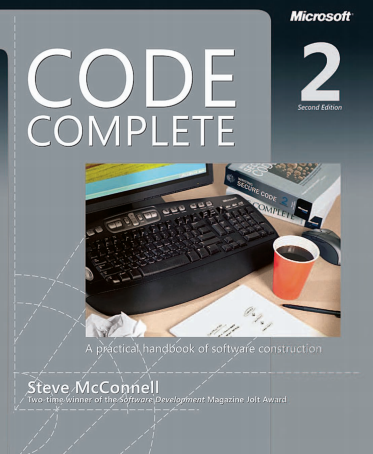
\includegraphics[width=0.5\textwidth]{codeCompleteCover.png}
\end{center}

Steve McConnell, Code Complete

\begin{center}
	
\includegraphics[width=0.5\textwidth]{cleanCodeCover.png}
\end{center}

Роберт Мартин, Чистый Код

\end{document}
